\section*{Описание экспериментальной установки}
\begin{figure}[H]
	\centering
	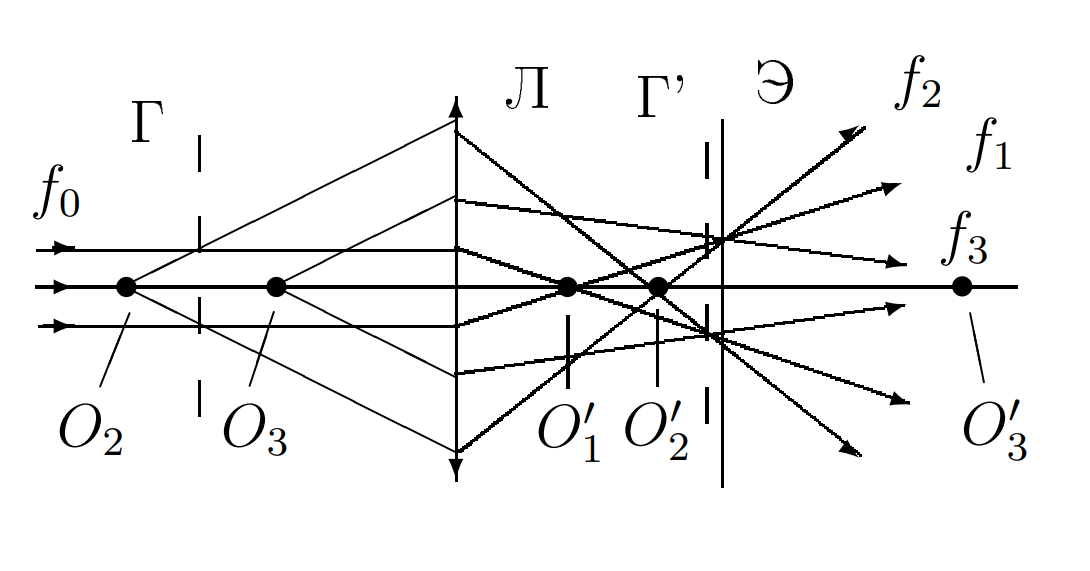
\includegraphics[width=1\textwidth]{../Изображения/Схема установки.png}
	\caption{Голограмма точечного источника}
\end{figure}

При просвечивании голограммы точечного источника плоской волной с амплитудой $f_{0} = const$, на выходе имеются три волны: плоская с амплитудой $f_{1} = const$, расходящаяся сферическая волна $f_{2} \propto e^{ikr}$, отвечающая мнимому изображению $O_{2}$, и сходящаяся сферическая волна $f_{3} \propto e^{-ikr}$, отвечающая действительному изображению $O_{3}$. После прохождения линзы Л волна $f_{1}$ собирается в фокусе линзы в точке ${O}'_{1}$, волны $f_{2}$ и $f_{3}$ фокусируются соответственно в точках ${O}'_{2}$ и ${O}'_{3}$. Изображение, возникающее на экране Э, можно рассматривать как результат интерференции сферических волн от трёх точечных источников ${O}'_{1}$, ${O}'_{2}$ и ${O}'_{3}$.

Кроме голограммы точечного источника в работе исследуется голограмма объёмного предмета, который представляет собой горизонтально расположенную миллиметровую линейку и вертикальный металлический стержень. При записи голограммы предмет распологался на расстоянии 10 см от пластинки. Голограмма установлена вертикально и может вращаться вокруг вертикальной оси. Источником света служит лазер длиной волны 532 нм и диаметром луча < 1мм. 